% Options for packages loaded elsewhere
% Options for packages loaded elsewhere
\PassOptionsToPackage{unicode}{hyperref}
\PassOptionsToPackage{hyphens}{url}
\PassOptionsToPackage{dvipsnames,svgnames,x11names}{xcolor}
%
\documentclass[
  spanish,
  us-letterpaper,
  DIV=11,
  numbers=noendperiod]{scrreprt}
\usepackage{xcolor}
\usepackage{amsmath,amssymb}
\setcounter{secnumdepth}{5}
\usepackage{iftex}
\ifPDFTeX
  \usepackage[T1]{fontenc}
  \usepackage[utf8]{inputenc}
  \usepackage{textcomp} % provide euro and other symbols
\else % if luatex or xetex
  \usepackage{unicode-math} % this also loads fontspec
  \defaultfontfeatures{Scale=MatchLowercase}
  \defaultfontfeatures[\rmfamily]{Ligatures=TeX,Scale=1}
\fi
\usepackage{lmodern}
\ifPDFTeX\else
  % xetex/luatex font selection
\fi
% Use upquote if available, for straight quotes in verbatim environments
\IfFileExists{upquote.sty}{\usepackage{upquote}}{}
\IfFileExists{microtype.sty}{% use microtype if available
  \usepackage[]{microtype}
  \UseMicrotypeSet[protrusion]{basicmath} % disable protrusion for tt fonts
}{}
\makeatletter
\@ifundefined{KOMAClassName}{% if non-KOMA class
  \IfFileExists{parskip.sty}{%
    \usepackage{parskip}
  }{% else
    \setlength{\parindent}{0pt}
    \setlength{\parskip}{6pt plus 2pt minus 1pt}}
}{% if KOMA class
  \KOMAoptions{parskip=half}}
\makeatother
% Make \paragraph and \subparagraph free-standing
\makeatletter
\ifx\paragraph\undefined\else
  \let\oldparagraph\paragraph
  \renewcommand{\paragraph}{
    \@ifstar
      \xxxParagraphStar
      \xxxParagraphNoStar
  }
  \newcommand{\xxxParagraphStar}[1]{\oldparagraph*{#1}\mbox{}}
  \newcommand{\xxxParagraphNoStar}[1]{\oldparagraph{#1}\mbox{}}
\fi
\ifx\subparagraph\undefined\else
  \let\oldsubparagraph\subparagraph
  \renewcommand{\subparagraph}{
    \@ifstar
      \xxxSubParagraphStar
      \xxxSubParagraphNoStar
  }
  \newcommand{\xxxSubParagraphStar}[1]{\oldsubparagraph*{#1}\mbox{}}
  \newcommand{\xxxSubParagraphNoStar}[1]{\oldsubparagraph{#1}\mbox{}}
\fi
\makeatother


\usepackage{longtable,booktabs,array}
\usepackage{calc} % for calculating minipage widths
% Correct order of tables after \paragraph or \subparagraph
\usepackage{etoolbox}
\makeatletter
\patchcmd\longtable{\par}{\if@noskipsec\mbox{}\fi\par}{}{}
\makeatother
% Allow footnotes in longtable head/foot
\IfFileExists{footnotehyper.sty}{\usepackage{footnotehyper}}{\usepackage{footnote}}
\makesavenoteenv{longtable}
\usepackage{graphicx}
\makeatletter
\newsavebox\pandoc@box
\newcommand*\pandocbounded[1]{% scales image to fit in text height/width
  \sbox\pandoc@box{#1}%
  \Gscale@div\@tempa{\textheight}{\dimexpr\ht\pandoc@box+\dp\pandoc@box\relax}%
  \Gscale@div\@tempb{\linewidth}{\wd\pandoc@box}%
  \ifdim\@tempb\p@<\@tempa\p@\let\@tempa\@tempb\fi% select the smaller of both
  \ifdim\@tempa\p@<\p@\scalebox{\@tempa}{\usebox\pandoc@box}%
  \else\usebox{\pandoc@box}%
  \fi%
}
% Set default figure placement to htbp
\def\fps@figure{htbp}
\makeatother



\ifLuaTeX
\usepackage[bidi=basic]{babel}
\else
\usepackage[bidi=default]{babel}
\fi
% get rid of language-specific shorthands (see #6817):
\let\LanguageShortHands\languageshorthands
\def\languageshorthands#1{}


\setlength{\emergencystretch}{3em} % prevent overfull lines

\providecommand{\tightlist}{%
  \setlength{\itemsep}{0pt}\setlength{\parskip}{0pt}}



 


\KOMAoption{captions}{tableheading}
\makeatletter
\@ifpackageloaded{bookmark}{}{\usepackage{bookmark}}
\makeatother
\makeatletter
\@ifpackageloaded{caption}{}{\usepackage{caption}}
\AtBeginDocument{%
\ifdefined\contentsname
  \renewcommand*\contentsname{Tabla de contenidos}
\else
  \newcommand\contentsname{Tabla de contenidos}
\fi
\ifdefined\listfigurename
  \renewcommand*\listfigurename{Listado de Figuras}
\else
  \newcommand\listfigurename{Listado de Figuras}
\fi
\ifdefined\listtablename
  \renewcommand*\listtablename{Listado de Tablas}
\else
  \newcommand\listtablename{Listado de Tablas}
\fi
\ifdefined\figurename
  \renewcommand*\figurename{Figura}
\else
  \newcommand\figurename{Figura}
\fi
\ifdefined\tablename
  \renewcommand*\tablename{Tabla}
\else
  \newcommand\tablename{Tabla}
\fi
}
\@ifpackageloaded{float}{}{\usepackage{float}}
\floatstyle{ruled}
\@ifundefined{c@chapter}{\newfloat{codelisting}{h}{lop}}{\newfloat{codelisting}{h}{lop}[chapter]}
\floatname{codelisting}{Listado}
\newcommand*\listoflistings{\listof{codelisting}{Listado de Listados}}
\makeatother
\makeatletter
\makeatother
\makeatletter
\@ifpackageloaded{caption}{}{\usepackage{caption}}
\@ifpackageloaded{subcaption}{}{\usepackage{subcaption}}
\makeatother
\usepackage{bookmark}
\IfFileExists{xurl.sty}{\usepackage{xurl}}{} % add URL line breaks if available
\urlstyle{same}
\hypersetup{
  pdftitle={Tesis},
  pdfauthor={Mariana Belén Cruz Rodríguez; Yofre Hernán García Gómez},
  pdflang={es},
  colorlinks=true,
  linkcolor={blue},
  filecolor={Maroon},
  citecolor={Blue},
  urlcolor={Blue},
  pdfcreator={LaTeX via pandoc}}


\title{Tesis}
\author{Mariana Belén Cruz Rodríguez \and Yofre Hernán García Gómez}
\date{}
\begin{document}
\maketitle

\renewcommand*\contentsname{Tabla de contenidos}
{
\hypersetup{linkcolor=}
\setcounter{tocdepth}{2}
\tableofcontents
}

\bookmarksetup{startatroot}

\chapter{Introducción}\label{introducciuxf3n}

En este trabajo se aborda el problema de \textbf{reconocimiento
automático de glifos del alfabeto náhuatl} mediante el uso de redes
neuronales convolucionales (\emph{Convolutional Neural Networks}, CNN).
Este problema puede formularse como una tarea de clasificación de
imágenes, en la cual cada glifo es representado mediante una estructura
matricial que codifica su información visual.

Los glifos presentan variaciones en forma, trazo y estilo, lo que
dificulta su identificación mediante métodos tradicionales. En este
contexto, las CNN resultan particularmente adecuadas debido a su
capacidad para extraer características espaciales relevantes
directamente a partir de los datos, tales como bordes, curvas y patrones
geométricos distintivos.

\bookmarksetup{startatroot}

\chapter{Formulación Matemática de una
CNN}\label{formulaciuxf3n-matemuxe1tica-de-una-cnn}

Una red neuronal convolucional puede modelarse como una aplicación
parametrizada:

\begin{equation}\phantomsection\label{eq-cnn-formal}{
f(\cdot , \theta): \mathcal{X} \subseteq \mathbb{R}^{H \times W \times C} \longrightarrow \mathbb{R}^{k}
}\end{equation}

donde:

\begin{itemize}
\tightlist
\item
  \(\mathcal{X}\) es el espacio de entrada (por ejemplo, imágenes),
\item
  \(H\) representa la altura (height) de la imagen, es decir, el número
  de filas,
\item
  \(W\) representa el ancho (width), es decir, el número de columnas,
\item
  \(C\) representa el número de canales (channels), que corresponde a la
  cantidad de valores asociados a cada píxel,
\item
  \(k\) es la dimensión del espacio de salida (por ejemplo, número de
  clases en clasificación),
\item
  \(\theta\) denota el conjunto total de parámetros entrenables del
  modelo.
\end{itemize}

\bookmarksetup{startatroot}

\chapter{Representación Tensorial de
Imágenes}\label{representaciuxf3n-tensorial-de-imuxe1genes}

Una imagen digital se representa como un tensor de orden tres:

\begin{equation}\phantomsection\label{eq-imagen-tensor}{
X \in \mathbb{R}^{H \times W \times C}
}\end{equation}

Esto implica que para cada posición espacial \((i,j)\):

\begin{equation}\phantomsection\label{eq-pixel-vector}{
X(i,j) = \left(x_1, x_2, \dots, x_C \right) \in \mathbb{R}^C
}\end{equation}

Por tanto, cada píxel contiene un vector que describe información en
distintos canales.

\pandocbounded{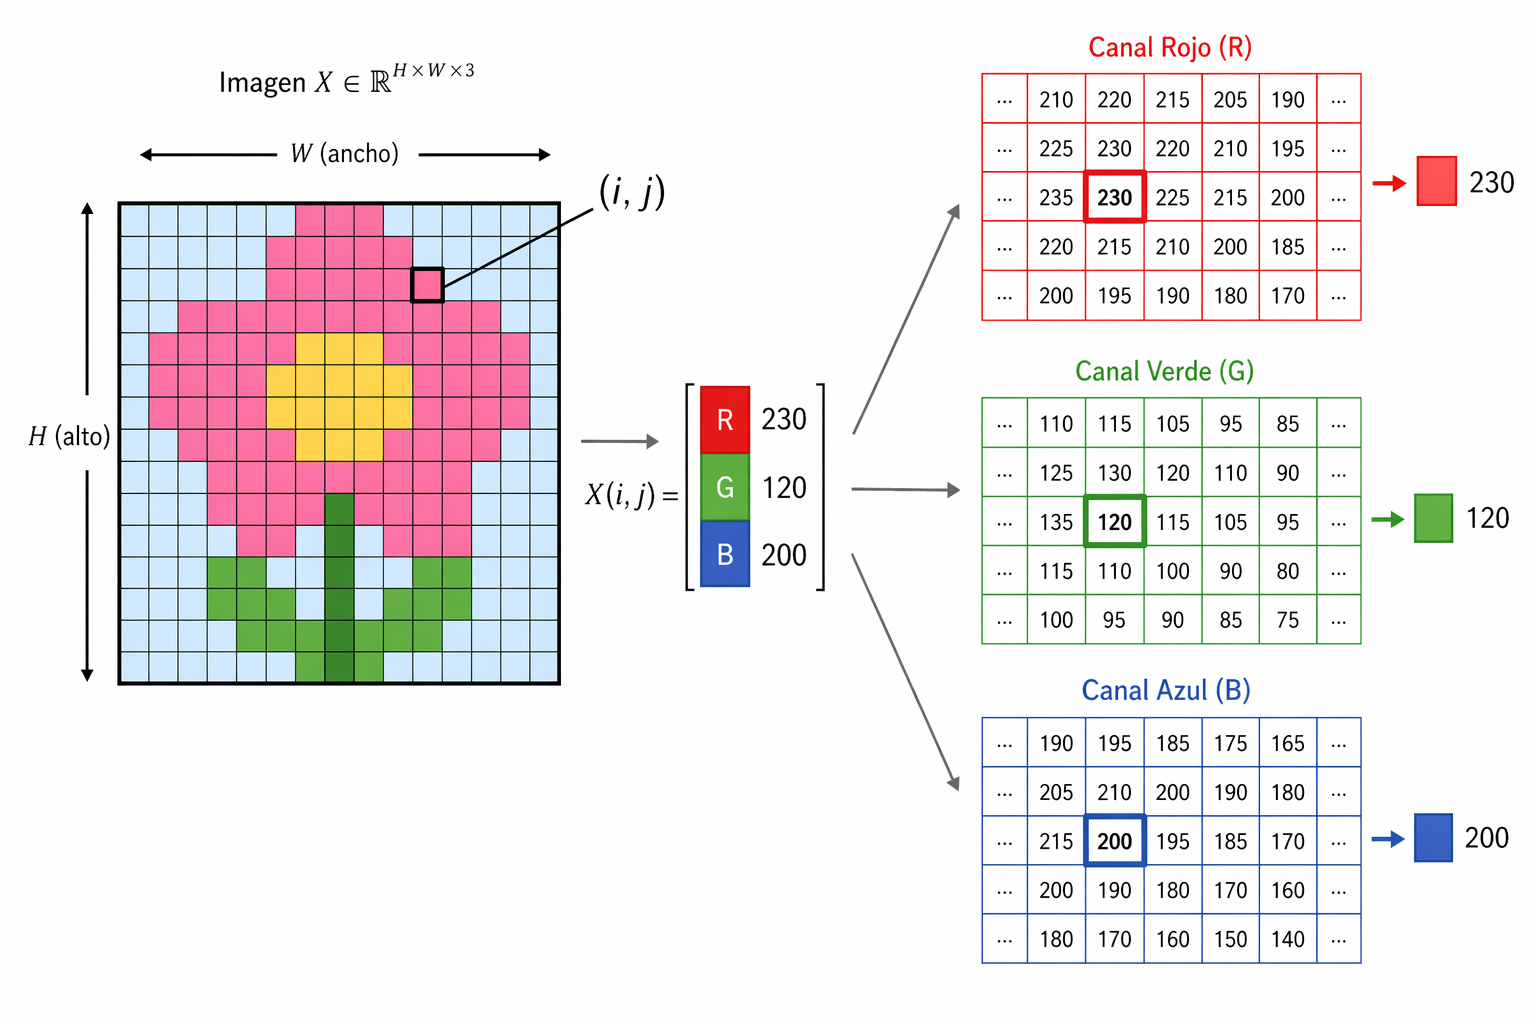
\includegraphics[keepaspectratio]{Imagenes_tesis/img_flor_1.png}}

\bookmarksetup{startatroot}

\chapter{Estructura Funcional de la
Red}\label{estructura-funcional-de-la-red}

Una CNN se construye como la composición de funciones:

\begin{equation}\phantomsection\label{eq-composicion-cnn}{
f(x;\theta) = f^{(L)} \circ f^{(L-1)} \circ \cdots \circ f^{(1)}(x)
}\end{equation}

donde \(L \in \mathbb{N}\) es el número total de capas de la red y cada
\(f^{(l)}\) representa una transformación asociada a la capa
\(l\)-ésima.

Asimismo, los parámetros globales se expresan como:

\begin{equation}\phantomsection\label{eq-parametros-globales}{
\theta = \left\{ \theta^{(1)}, \theta^{(2)}, \dots, \theta^{(L)} \right\}
}\end{equation}

\bookmarksetup{startatroot}

\chapter{Parámetros del Modelo}\label{paruxe1metros-del-modelo}

Los parámetros de una CNN están constituidos principalmente por:

\begin{itemize}
\tightlist
\item
  \textbf{Kernels} (filtros convolucionales),
\item
  \textbf{Sesgos} asociados a cada filtro.
\end{itemize}

Estos parámetros determinan completamente la función \(f(x;\theta)\) y
son ajustados mediante procedimientos de optimización basados en
gradiente.

\bookmarksetup{startatroot}

\chapter{Kernels Convolucionales}\label{kernels-convolucionales}

\section{Definición Formal}\label{definiciuxf3n-formal}

Un kernel es un tensor de parámetros que define un operador lineal
local.

\textbf{Caso unicanal:}

\begin{equation}\phantomsection\label{eq-kernel-unicanal}{
K \in \mathbb{R}^{k_h \times k_w}
}\end{equation}

cuyos elementos se indexan como:

\[
K(u,v), \quad
u \in \{0,\dots,k_h-1\}, \;
v \in \{0,\dots,k_w-1\}
\]

\textbf{Caso multicanal:}

\begin{equation}\phantomsection\label{eq-kernel-multicanal}{
K \in \mathbb{R}^{k_h \times k_w \times C}
}\end{equation}

con entradas:

\[
K(u,v,c), \quad
u \in \{0,\dots,k_h-1\}, \;
v \in \{0,\dots,k_w-1\}, \;
c \in \{1,\dots,C\}
\]

\section{Interpretación
Geométrica}\label{interpretaciuxf3n-geomuxe9trica}

Sea \(X_{(i,j)}\) una subregión de la imagen obtenida al centrar el
kernel en la posición \((i,j)\), cuyos elementos están dados por:

\[
X(i+u, j+v, c)
\]

para los mismos índices \((u,v,c)\) definidos anteriormente.

El producto interno:

\begin{equation}\phantomsection\label{eq-producto-interno}{
\langle K, X_{(i,j)} \rangle
}\end{equation}

mide la similitud entre el patrón definido por el kernel y la región
local de la imagen.

\pandocbounded{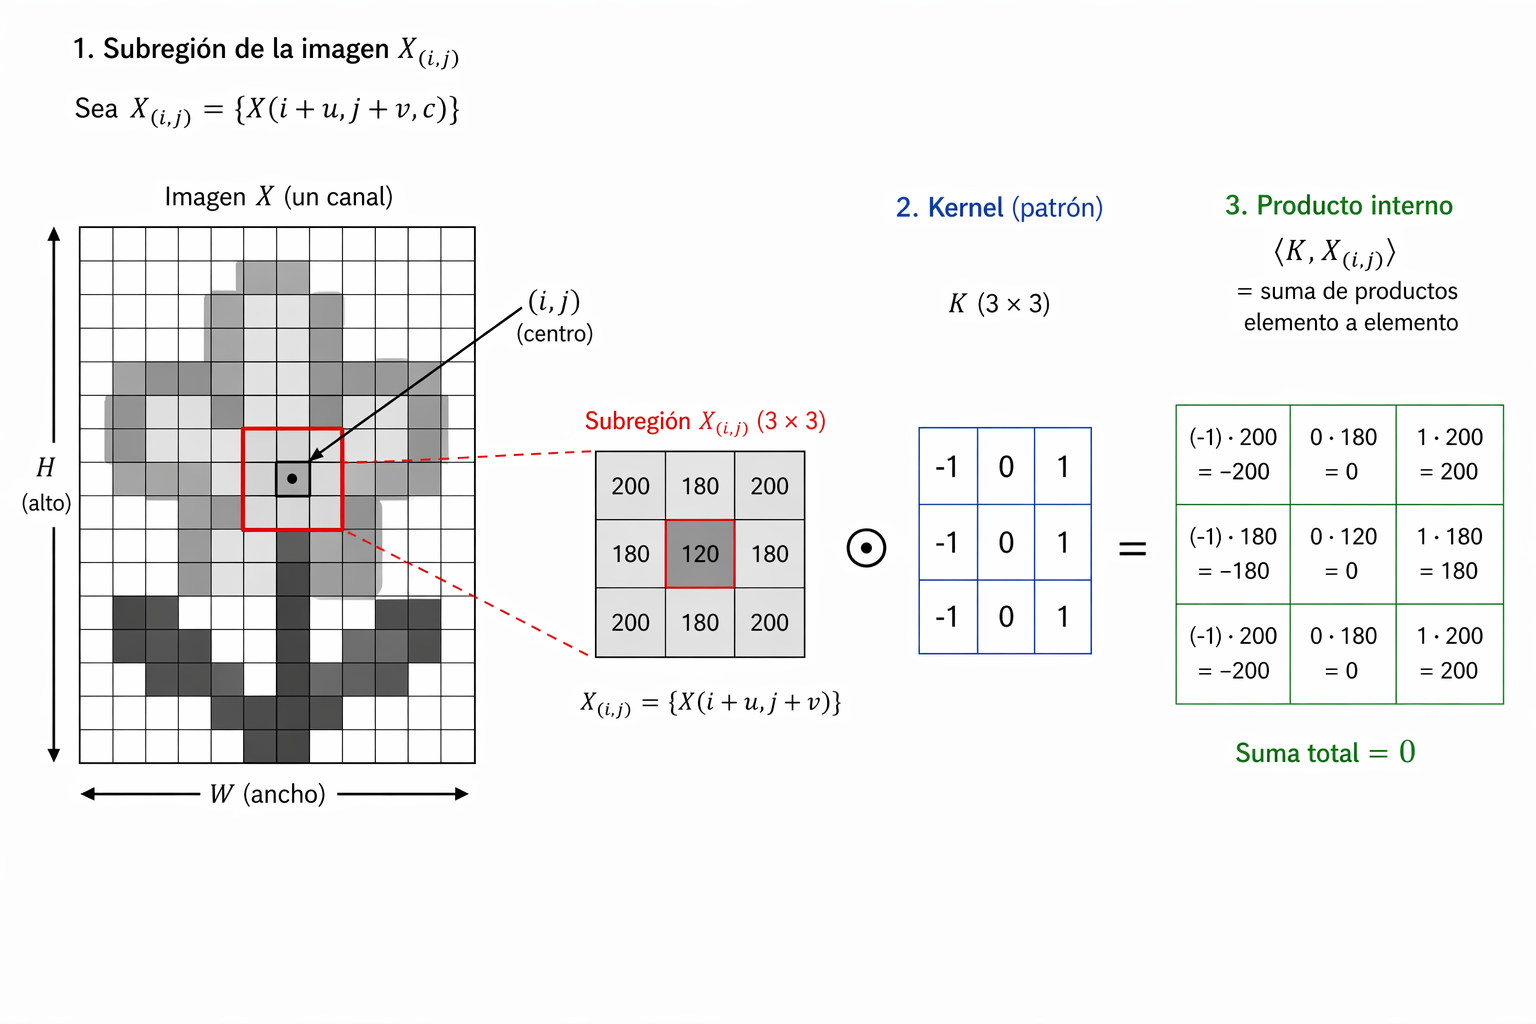
\includegraphics[keepaspectratio]{Imagenes_tesis/img_flor_2.png}}

\section{Compartición de
parámetros}\label{comparticiuxf3n-de-paruxe1metros}

Una propiedad fundamental de las redes neuronales convolucionales es la
\textbf{compartición de parámetros}, la cual establece que los
coeficientes del kernel no dependen de la posición espacial en la que se
aplica la operación.

Formalmente, si \(K\) es un kernel convolucional, entonces:

\[
K(u,v,c) \text{ es independiente de la posición } (i,j)
\]

Esto implica que el mismo kernel es utilizado para procesar todas las
regiones locales de la entrada.

\subsection{Reducción del número de
parámetros}\label{reducciuxf3n-del-nuxfamero-de-paruxe1metros}

En ausencia de compartición de parámetros, cada posición \((i,j)\)
requeriría un conjunto distinto de pesos, lo cual conduciría a un número
total de parámetros del orden:

\[
H \cdot W \cdot k_h \cdot k_w \cdot C
\]

Sin embargo, al emplear un único kernel compartido, el número de
parámetros se reduce a:

\[
k_h \cdot k_w \cdot C
\]

lo cual representa una reducción significativa en la complejidad del
modelo.

\subsection{Invarianza traslacional}\label{invarianza-traslacional}

La compartición de parámetros induce una propiedad de
\textbf{equivarianza por traslación}. Sea \(\tau_{a,b}\) un operador de
traslación definido sobre la entrada. Entonces, la operación de
convolución satisface:

\begin{equation}\phantomsection\label{eq-equivarianza}{
\mathcal{T}_K(\tau_{a,b} X) = \tau_{a,b} (\mathcal{T}_K X)
}\end{equation}

Esto implica que si una característica aparece en diferentes posiciones
espaciales, el modelo será capaz de detectarla de manera consistente.

En consecuencia, la red no depende de la posición absoluta de los
patrones, sino únicamente de su estructura local.

\bookmarksetup{startatroot}

\chapter{Operación de Convolución}\label{operaciuxf3n-de-convoluciuxf3n}

La operación fundamental en una red neuronal convolucional es la
denominada \textbf{convolución discreta}. No obstante, es importante
señalar que en el contexto de aprendizaje profundo, la operación
implementada corresponde en realidad a la \textbf{correlación cruzada},
ya que no se realiza la inversión del kernel. A pesar de esta diferencia
técnica, en la literatura se mantiene el término ``convolución'\,' por
convención.

Esta operación define un mecanismo mediante el cual se evalúa la
similitud entre un patrón local (kernel) y distintas regiones de la
imagen de entrada.

\section{Caso Unicanal}\label{caso-unicanal}

Sea una imagen unicanal representada por:

\[
X \in \mathbb{R}^{H \times W}
\]

y un kernel:

\[
K \in \mathbb{R}^{k_h \times k_w}
\]

La operación de convolución produce una salida \(Y\), definida en cada
posición \((i,j)\) como:

\begin{equation}\phantomsection\label{eq-convolucion-unicanal}{
Y(i,j) =
\sum_{u=0}^{k_h-1}
\sum_{v=0}^{k_w-1}
K(u,v)\, X(i+u, j+v)
}\end{equation}

donde:

\begin{itemize}
\tightlist
\item
  \((i,j)\) denota la posición de la ventana deslizante,
\item
  \((u,v)\) recorre las coordenadas internas del kernel,
\item
  \(X(i+u, j+v)\) representa la región local de la imagen.
\end{itemize}

\pandocbounded{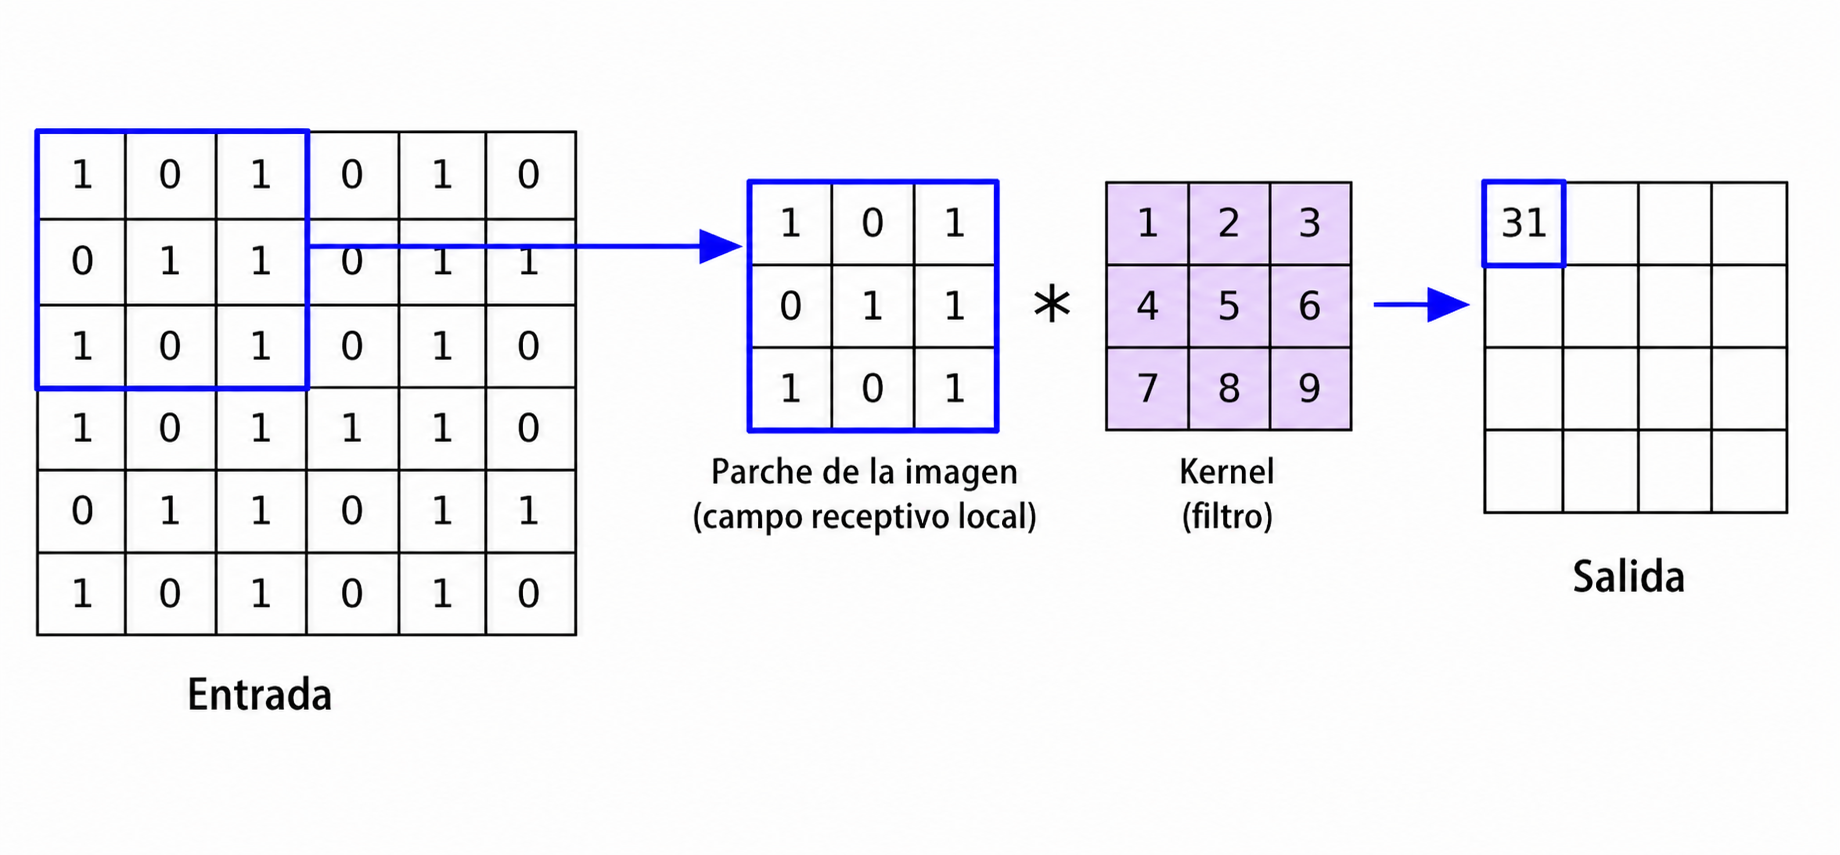
\includegraphics[keepaspectratio]{Imagenes_tesis/img_kernel_1.png}}

\subsection{Interpretación como ventana
deslizante}\label{interpretaciuxf3n-como-ventana-deslizante}

La ecuación anterior describe un proceso en el cual el kernel se
desplaza sistemáticamente sobre la imagen. En cada posición, se
selecciona una submatriz de \(X\) de dimensiones \(k_h \times k_w\),
sobre la cual se realiza una operación de agregación ponderada.

Formalmente, definimos la submatriz local como:

\[
X_{(i,j)} = \left\{ X(i+u, j+v) \right\}_{u,v}
\]

Por lo tanto, la salida en \((i,j)\) depende únicamente de una vecindad
local de la imagen, lo cual establece la propiedad de
\textbf{conectividad local}.

\subsection{Interpretación como producto
interno}\label{interpretaciuxf3n-como-producto-interno}

La expresión de la convolución puede reescribirse como un producto
interno en el espacio vectorial \(\mathbb{R}^{k_h \times k_w}\):

\begin{equation}\phantomsection\label{eq-producto-interno-conv}{
Y(i,j) = \langle K, X_{(i,j)} \rangle
}\end{equation}

donde el producto interno se define como:

\[
\langle A, B \rangle = \sum_{u=0}^{k_h-1} \sum_{v=0}^{k_w-1} A(u,v)\, B(u,v)
\]

Esta formulación pone de manifiesto que la convolución mide el grado de
alineación entre el kernel y la región local.

\subsection{Interpretación
geométrica}\label{interpretaciuxf3n-geomuxe9trica-1}

Desde un punto de vista geométrico, el valor \(Y(i,j)\) representa la
proyección del vector \(X_{(i,j)}\) sobre el vector \(K\) en el espacio
euclidiano de dimensión \(k_h k_w\). En consecuencia:

\begin{itemize}
\tightlist
\item
  Si \(X_{(i,j)}\) es similar a \(K\), entonces \(Y(i,j)\) será grande.
\item
  Si son ortogonales, el resultado será cercano a cero.
\item
  Si son opuestos, el valor será negativo.
\end{itemize}

Esto permite interpretar al kernel como un \textbf{detector de
patrones}.

\subsection{Naturaleza lineal de la
operación}\label{naturaleza-lineal-de-la-operaciuxf3n}

La convolución es un operador lineal. Es decir, para cualesquiera
tensores \(X_1, X_2\) y escalares \(\alpha, \beta\), se cumple:

\begin{equation}\phantomsection\label{eq-linealidad}{
\mathcal{T}_K(\alpha X_1 + \beta X_2)
= \alpha \mathcal{T}_K(X_1) + \beta \mathcal{T}_K(X_2)
}\end{equation}

donde \(\mathcal{T}_K\) denota el operador de convolución asociado al
kernel \(K\).

\subsection{Relación con la correlación
cruzada}\label{relaciuxf3n-con-la-correlaciuxf3n-cruzada}

Es importante destacar que la definición utilizada en redes neuronales
corresponde a la correlación cruzada:

\[
Y(i,j) =
\sum_{u,v} K(u,v)\, X(i+u, j+v)
\]

mientras que la convolución clásica implicaría una inversión del kernel:

\[
Y(i,j) =
\sum_{u,v} K(u,v)\, X(i-u, j-v)
\]

Sin embargo, dado que los parámetros del kernel son aprendidos durante
el entrenamiento, ambas formulaciones resultan equivalentes en términos
de capacidad representacional.

\subsection{Dependencia local}\label{dependencia-local}

Finalmente, se observa que:

\[
Y(i,j) \text{ depende únicamente de } X_{(i,j)}
\]

lo cual implica que cada salida está influenciada únicamente por una
región local de la entrada. Esta propiedad es clave para la eficiencia
computacional y la capacidad de generalización del modelo.

\section{Convolución Multicanal}\label{convoluciuxf3n-multicanal}

En el caso general, las imágenes no son unicanal, sino que poseen
múltiples canales (por ejemplo, RGB). En consecuencia, la operación de
convolución debe extenderse para considerar simultáneamente la
información presente en cada canal.

Sea:

\[
X \in \mathbb{R}^{H \times W \times C}
\]

una imagen con \(C\) canales, y sea un kernel:

\[
K \in \mathbb{R}^{k_h \times k_w \times C}
\]

donde cada canal del kernel corresponde a un canal de la entrada.

La salida de la convolución en la posición \((i,j)\) está dada por:

\begin{equation}\phantomsection\label{eq-convolucion-multicanal}{
Y(i,j) =
\sum_{c=1}^{C}
\sum_{u=0}^{k_h-1}
\sum_{v=0}^{k_w-1}
K(u,v,c)\, X(i+u,j+v,c)
}\end{equation}

Esta expresión indica que la contribución de cada canal se calcula de
manera independiente y posteriormente se agregan (suman) todas las
contribuciones.

La operación anterior puede interpretarse como la suma de convoluciones
unicanal:

\[
Y(i,j) = \sum_{c=1}^{C} Y^{(c)}(i,j)
\]

donde:

\[
Y^{(c)}(i,j) =
\sum_{u=0}^{k_h-1}
\sum_{v=0}^{k_w-1}
K(u,v,c)\, X(i+u,j+v,c)
\]

Cada término \(Y^{(c)}(i,j)\) representa la contribución del canal \(c\)
al valor final de la salida.

\pandocbounded{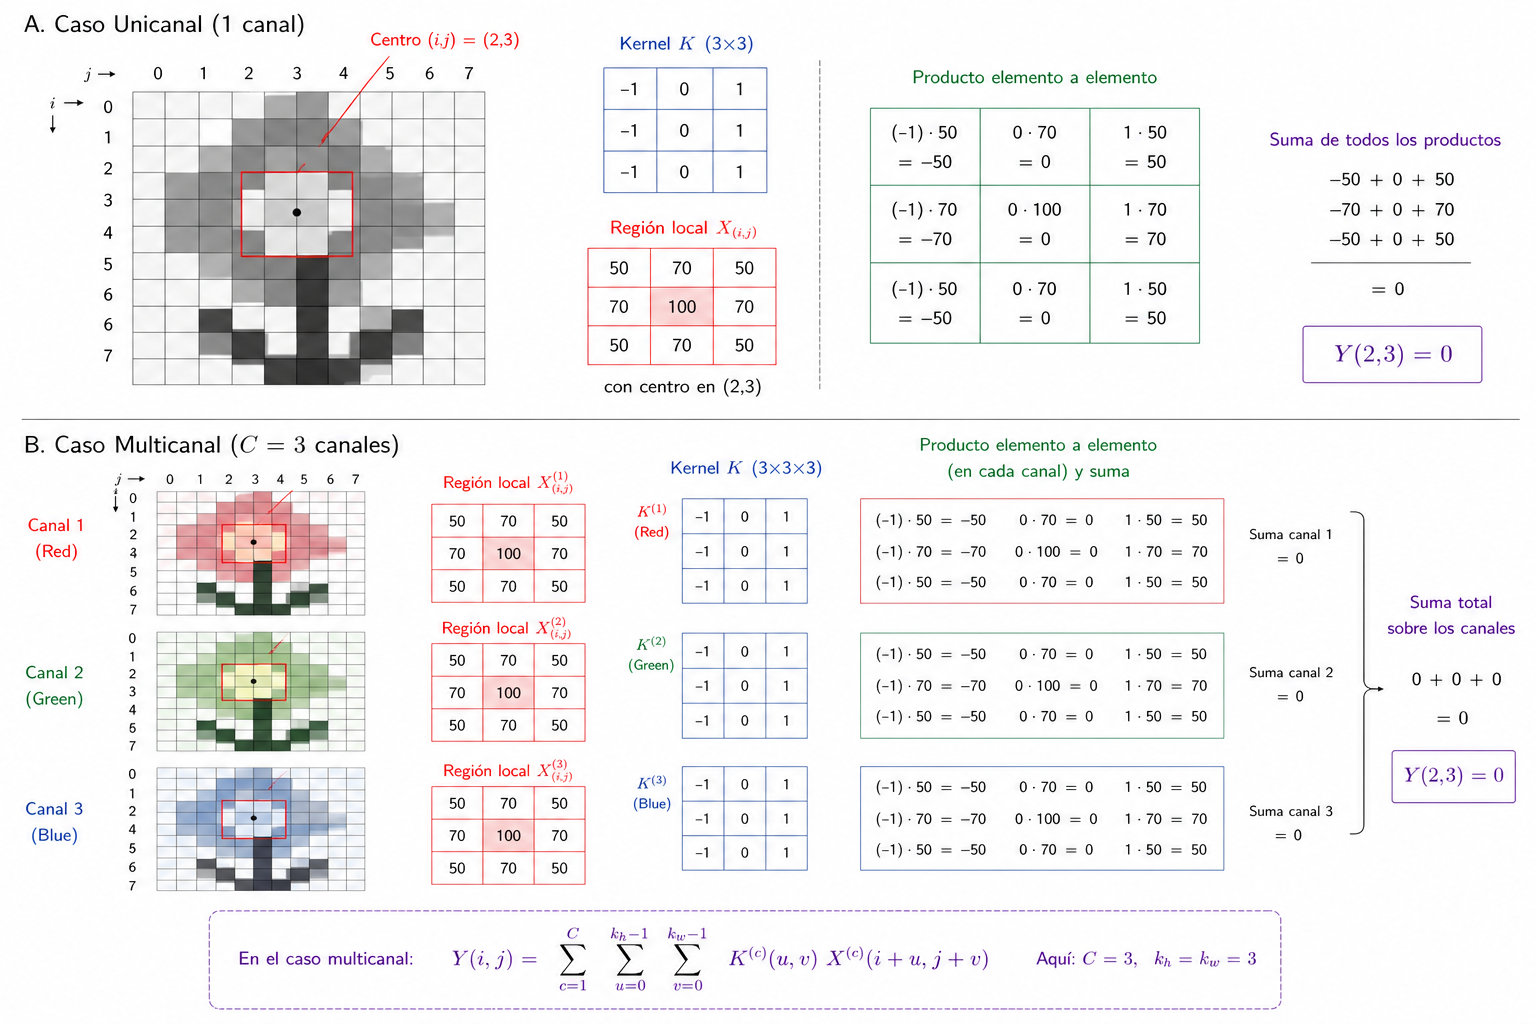
\includegraphics[keepaspectratio]{Imagenes_tesis/imagen_provicional.png.png}}

\section{Interpretación como producto interno en espacio
tensorial}\label{interpretaciuxf3n-como-producto-interno-en-espacio-tensorial}

Sea \(X_{(i,j)}\) la subregión local de la imagen centrada en \((i,j)\).
Entonces:

\[
X_{(i,j)} \in \mathbb{R}^{k_h \times k_w \times C}
\]

Al vectorizar ambos tensores:

\[
\mathrm{vec}(X_{(i,j)}) \in \mathbb{R}^{k_h k_w C}, \quad
\mathrm{vec}(K) \in \mathbb{R}^{k_h k_w C}
\]

la convolución puede escribirse como:

\begin{equation}\phantomsection\label{eq-vectorizacion}{
Y(i,j) = \mathrm{vec}(K)^\top \mathrm{vec}(X_{(i,j)})
}\end{equation}

Esto muestra que la operación es un producto interno en un espacio
euclidiano de dimensión \(k_h k_w C\).

\section{Interpretación
geométrica}\label{interpretaciuxf3n-geomuxe9trica-2}

Desde un punto de vista geométrico, cada región local de la imagen se
interpreta como un punto en el espacio \(\mathbb{R}^{k_h k_w C}\), y el
kernel define una dirección en dicho espacio.

Por tanto:

\begin{itemize}
\tightlist
\item
  valores grandes de \(Y(i,j)\) indican alta alineación entre el patrón
  y la región,
\item
  valores cercanos a cero indican baja correlación,
\item
  valores negativos indican oposición estructural.
\end{itemize}

En consecuencia, el kernel actúa como un detector de patrones
multicanal.

\section{Naturaleza lineal}\label{naturaleza-lineal}

La convolución multicanal es un operador lineal. Es decir, para
cualesquiera tensores \(X_1, X_2\) y escalares \(\alpha, \beta\), se
cumple:

\[
\mathcal{T}_K(\alpha X_1 + \beta X_2)
=
\alpha \mathcal{T}_K(X_1) + \beta \mathcal{T}_K(X_2)
\]

donde \(\mathcal{T}_K\) denota el operador de convolución asociado al
kernel \(K\).

\section{Interpretación
estructural}\label{interpretaciuxf3n-estructural}

Es importante destacar que, a diferencia del caso unicanal, el kernel
multicanal no detecta únicamente patrones espaciales, sino también
\textbf{correlaciones entre canales}.

Por ejemplo, en imágenes RGB, el kernel puede aprender a identificar
combinaciones específicas de intensidades en los canales rojo, verde y
azul, lo cual permite detectar patrones más complejos que aquellos
basados únicamente en estructura espacial.

\section{Forma Vectorizada}\label{forma-vectorizada}

\[
Y(i,j) = K^\top X_{(i,j)}
\]

\bookmarksetup{startatroot}

\chapter{Múltiples Filtros}\label{muxfaltiples-filtros}

En una red neuronal convolucional, no se utiliza un único kernel, sino
un conjunto de filtros que permiten extraer distintas características de
la entrada. Este conjunto se denota como:

\begin{equation}\phantomsection\label{eq-conjunto-filtros}{
\left\{ K^{(f)} \right\}_{f=1}^{F}, \quad
K^{(f)} \in \mathbb{R}^{k_h \times k_w \times C}
}\end{equation}

donde \(F\) representa el número total de filtros.

\section{Definición de la salida}\label{definiciuxf3n-de-la-salida}

Cada filtro \(K^{(f)}\) actúa de manera independiente sobre la entrada y
produce un mapa de activación asociado. Para cada posición \((i,j)\), la
salida correspondiente al filtro \(f\) está dada por:

\begin{equation}\phantomsection\label{eq-salida-filtro}{
Y_f(i,j) = \langle K^{(f)}, X_{(i,j)} \rangle
}\end{equation}

Por lo tanto, a cada filtro le corresponde una función:

\[
Y_f : \{1,\dots,H'\} \times \{1,\dots,W'\} \to \mathbb{R}
\]

\section{Estructura tensorial de la
salida}\label{estructura-tensorial-de-la-salida}

Al considerar todos los filtros simultáneamente, la salida completa se
organiza como un tensor de orden tres:

\begin{equation}\phantomsection\label{eq-salida-tensor}{
Y \in \mathbb{R}^{H' \times W' \times F}
}\end{equation}

donde:

\begin{itemize}
\tightlist
\item
  \(H'\) y \(W'\) son las dimensiones espaciales de la salida,
\item
  \(F\) es el número de canales de salida, también llamados
  \textbf{mapas de características}.
\end{itemize}

En particular, la componente \(Y(:,:,f)\) corresponde al mapa de
activación generado por el filtro \(K^{(f)}\).

\section{Interpretación funcional}\label{interpretaciuxf3n-funcional}

Cada filtro puede interpretarse como un detector especializado en cierto
tipo de patrón. En consecuencia, la colección de filtros define una
familia de funciones:

\[
\left\{ \mathcal{T}_{K^{(f)}} \right\}_{f=1}^{F}
\]

donde cada operador \(\mathcal{T}_{K^{(f)}}\) extrae una característica
distinta de la entrada.

De este modo, la salida de la capa puede interpretarse como la
aplicación conjunta de múltiples detectores, produciendo una
representación enriquecida de la imagen.

\section{Interpretación como vector de características
local}\label{interpretaciuxf3n-como-vector-de-caracteruxedsticas-local}

Para cada posición \((i,j)\), la salida puede agruparse como un vector:

\begin{equation}\phantomsection\label{eq-vector-local}{
Y(i,j) = \left( Y_1(i,j), Y_2(i,j), \dots, Y_F(i,j) \right) \in \mathbb{R}^{F}
}\end{equation}

Esto implica que cada posición espacial de la imagen original es
transformada en un vector de características de dimensión \(F\).

Por tanto, la capa convolucional realiza una transformación:

\[
\mathbb{R}^{k_h \times k_w \times C}
\longrightarrow
\mathbb{R}^{F}
\]

aplicada localmente en cada vecindad de la imagen.

\section{Interpretación
geométrica}\label{interpretaciuxf3n-geomuxe9trica-3}

Desde una perspectiva geométrica, cada filtro \(K^{(f)}\) define una
dirección en el espacio \(\mathbb{R}^{k_h k_w C}\). En consecuencia, el
vector \(Y(i,j)\) contiene las proyecciones de la región local
\(X_{(i,j)}\) sobre cada una de estas direcciones.

Esto permite interpretar la salida como una representación de la
información local en una base (no necesariamente ortogonal) definida por
los filtros aprendidos.

\section{Ejemplos de filtros}\label{ejemplos-de-filtros}

Los distintos filtros convolucionales permiten detectar características
específicas en la imagen de entrada. A continuación, se muestran
ejemplos representativos del efecto de diferentes kernels sobre una
misma imagen.

\begin{figure}[H]

{\centering \pandocbounded{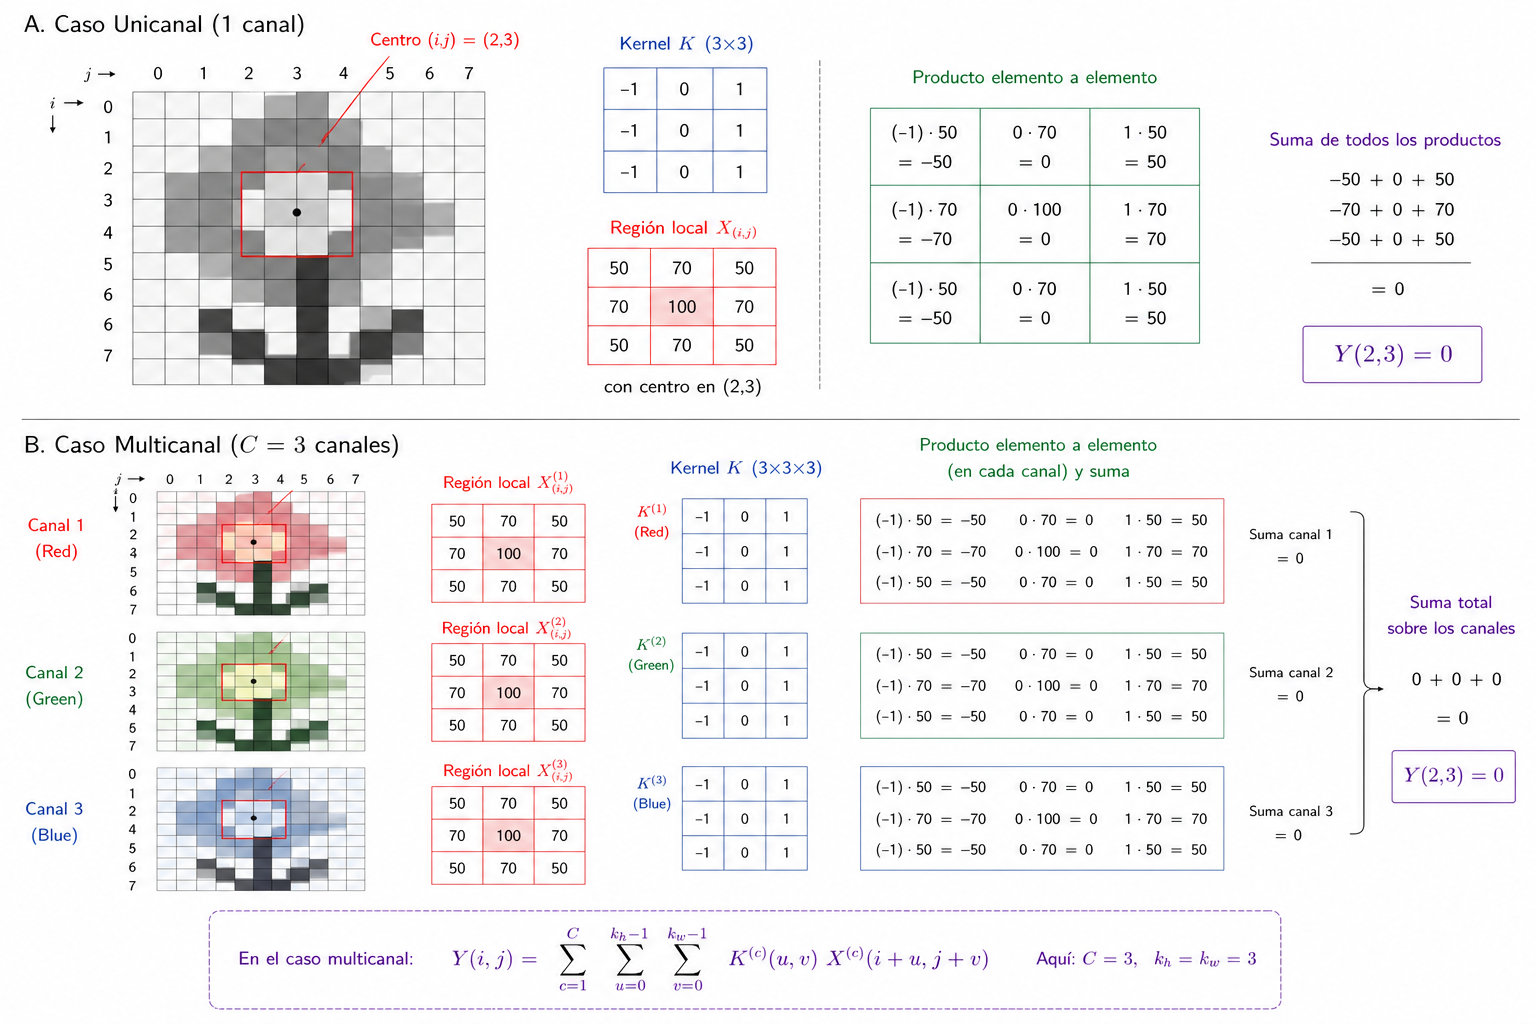
\includegraphics[keepaspectratio]{Imagenes_tesis/imagen_provicional.png}}

}

\caption{Efecto de distintos filtros convolucionales sobre una imagen}

\end{figure}%

\section{Observación estructural}\label{observaciuxf3n-estructural}

Es importante notar que el número de filtros \(F\) determina la
capacidad de representación de la capa. Un mayor número de filtros
permite capturar una mayor variedad de patrones, pero también incrementa
el número de parámetros y el costo computacional.

En capas profundas, los filtros tienden a representar características de
mayor nivel semántico, construidas a partir de combinaciones de patrones
detectados en capas anteriores.

\bookmarksetup{startatroot}

\chapter{Stride y Padding}\label{stride-y-padding}

\section{Stride}\label{stride}

El \emph{stride} \(s\) controla el desplazamiento del kernel durante la
operación de convolución. Es decir, determina cuántas posiciones se
desplaza el kernel en cada paso.

Las dimensiones de salida están dadas por:

\begin{equation}\phantomsection\label{eq-output-dims}{
H' = \left\lfloor \frac{H - k_h + 2p}{s} \right\rfloor + 1, \quad
W' = \left\lfloor \frac{W - k_w + 2p}{s} \right\rfloor + 1
}\end{equation}

donde:

\begin{itemize}
\tightlist
\item
  \(H, W\) son las dimensiones de la entrada,
\item
  \(k_h, k_w\) son las dimensiones del kernel,
\item
  \(p\) es el padding,
\item
  \(s\) es el stride.
\end{itemize}

Un valor mayor de \(s\) produce una reducción en la resolución espacial
de la salida.

\section{Padding}\label{padding}

El \emph{padding} es una operación que consiste en añadir valores
(generalmente ceros) alrededor de la entrada antes de aplicar la
convolución. Esto se hace para controlar el tamaño de la salida y
preservar información en los bordes.

\[
X_{\text{pad}} \in \mathbb{R}^{(H+2p)\times(W+2p)\times C}
\]

El padding puede interpretarse como una extensión de la función de
entrada \(X\) fuera de su dominio original. Formalmente, se define la
extensión \(\tilde{X}\) como:

\[
\tilde{X}(i,j) =
\begin{cases}
X(i,j), & \text{si } (i,j) \text{ pertenece al dominio original}, \\
0, & \text{en otro caso}
\end{cases}
\]

Esta extensión corresponde a una extensión por cero del dominio de la
función.

En una capa convolucional, el padding se aplica antes de la convolución.
Por lo tanto, la operación completa de una capa convolucional con
padding se puede expresar como:

\[
Y = \sigma\big( (\text{pad}(X)) \star K + b \big)
\]

donde:

\begin{itemize}
\tightlist
\item
  \(X\) es el tensor de entrada,
\item
  \(\text{pad}(X)\) es la entrada extendida mediante padding,
\item
  \(\star\) denota la operación de correlación cruzada,
\item
  \(K\) es el kernel o filtro,
\item
  \(b\) es el sesgo,
\item
  \(\sigma\) es la función de activación.
\end{itemize}

\section{Ejemplo ilustrativo}\label{ejemplo-ilustrativo}

Para ilustrar el efecto del padding sobre las dimensiones de salida, se
presenta el siguiente ejemplo:

\begin{figure}

\centering{

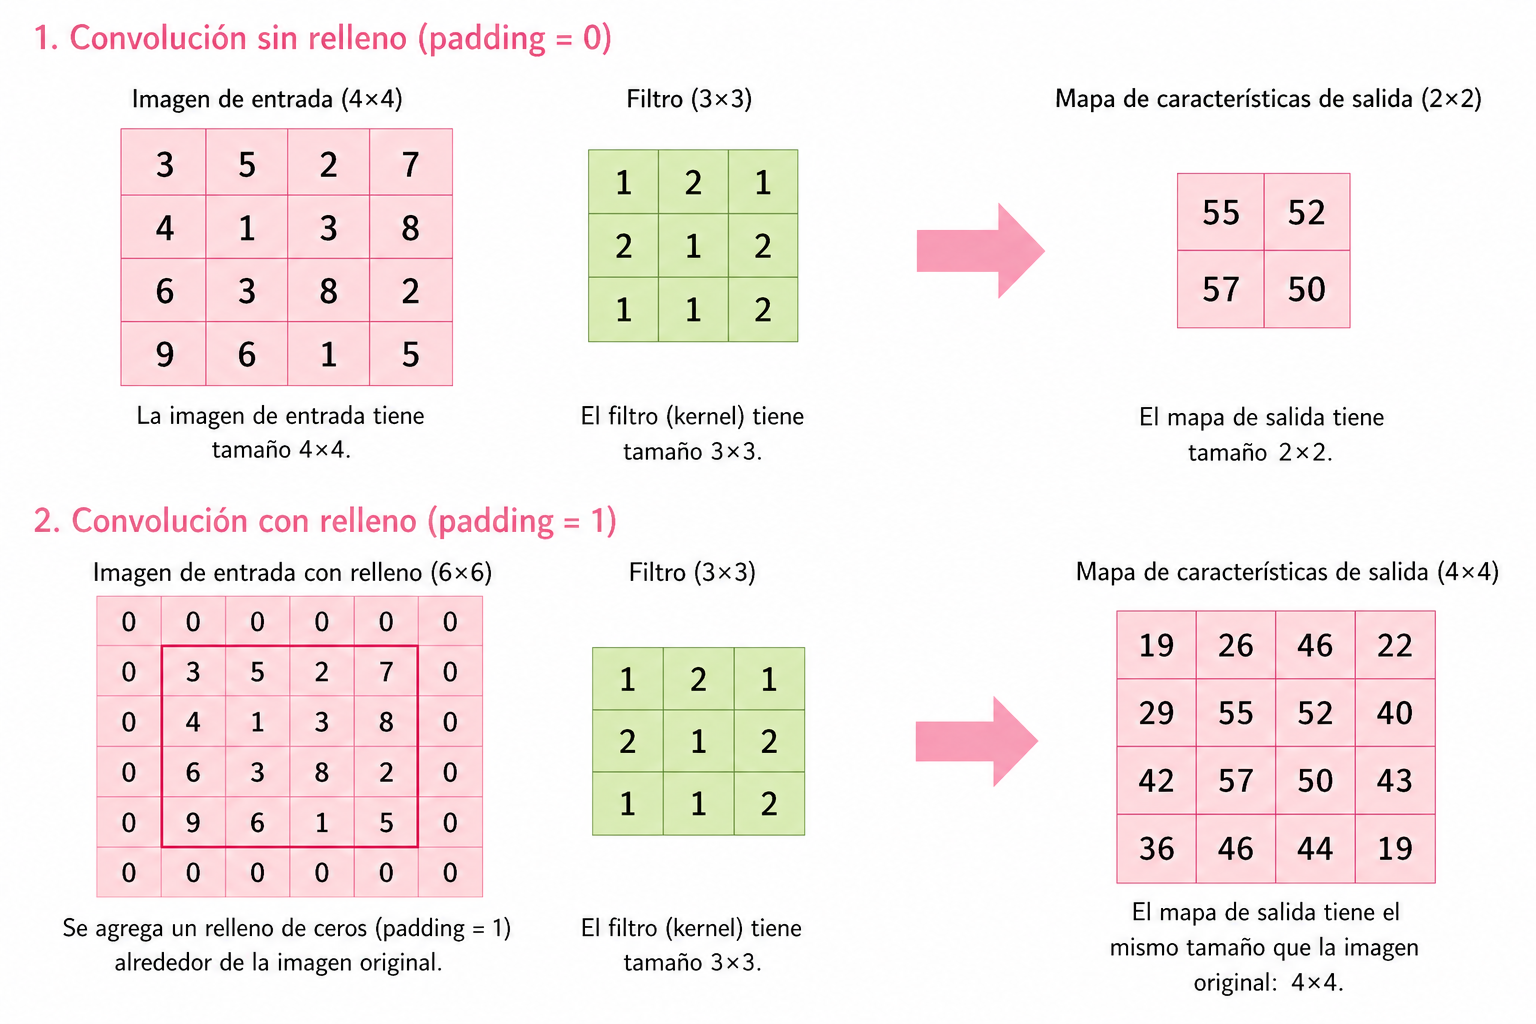
\includegraphics[width=0.8\linewidth,height=\textheight,keepaspectratio]{Imagenes_tesis/img_kernel_mapa.png}

}

\caption{\label{fig-padding}Ejemplo de convolución con y sin padding}

\end{figure}%

Como se observa en Figura~\ref{fig-padding}, la incorporación de padding
permite controlar el tamaño de la salida. En particular, cuando se
utiliza padding adecuado, es posible preservar las dimensiones
espaciales de la imagen original tras la aplicación de la convolución.

\section{Función de activación}\label{funciuxf3n-de-activaciuxf3n}

Una función de activación es una aplicación no lineal que se introduce
después de una transformación afín, con el objetivo de dotar al modelo
de la capacidad de aproximar funciones no lineales.

\subsection{Definición}\label{definiciuxf3n}

Sea \(x \in \mathbb{R}^n\) un vector de entrada, \(w \in \mathbb{R}^n\)
un vector de pesos y \(b \in \mathbb{R}\) un sesgo. Se define la
preactivación como:

\begin{equation}\phantomsection\label{eq-preactivacion}{
z = w^T x + b
}\end{equation}

La salida de la neurona está dada por:

\begin{equation}\phantomsection\label{eq-activacion}{
y = \sigma(z)
}\end{equation}

donde \(\sigma : \mathbb{R} \to \mathbb{R}\) es la función de
activación.

\subsection{No linealidad}\label{no-linealidad}

Considérese una red neuronal profunda compuesta únicamente por
transformaciones afines. En tal caso, la composición de dichas
transformaciones satisface:

\[
f(x) = W_L W_{L-1} \cdots W_1 x + b'
\]

lo cual sigue siendo una transformación afín. Por consiguiente, sin la
introducción de funciones de activación no lineales, la red carece de
capacidad expresiva para modelar relaciones no lineales.

En una red neuronal convolucional (CNN), la salida de una capa se
expresa como:

\begin{equation}\phantomsection\label{eq-cnn-activacion}{
Y = \sigma\big( X \star K + b \big)
}\end{equation}

donde:

\begin{itemize}
\tightlist
\item
  \(X\) es el tensor de entrada\\
\item
  \(\star\) denota la operación de correlación cruzada\\
\item
  \(K\) es el conjunto de filtros (kernels)\\
\item
  \(b\) es el sesgo\\
\item
  \(\sigma\) se aplica elemento a elemento
\end{itemize}

\subsection{Ejemplos de funciones de
activación}\label{ejemplos-de-funciones-de-activaciuxf3n}

Algunas de las funciones de activación más utilizadas son las
siguientes: \begin{center}
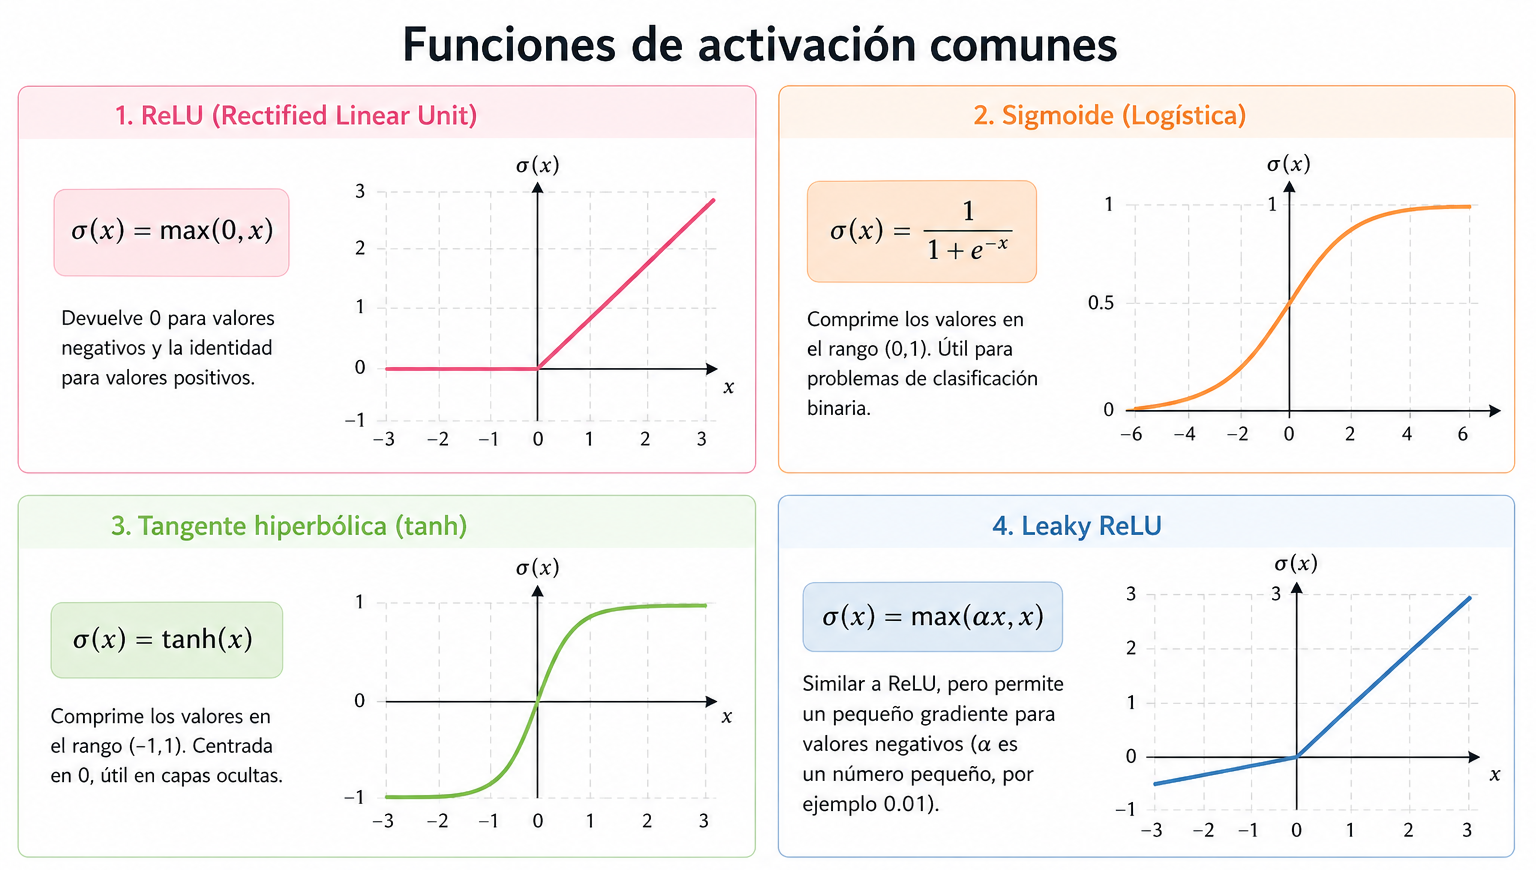
\includegraphics[width=0.8\linewidth,height=\textheight,keepaspectratio]{Imagenes_tesis/img_funciones_activacion.png}
\end{center}

\subsubsection{ReLU (Rectified Linear
Unit)}\label{relu-rectified-linear-unit}

\begin{equation}\phantomsection\label{eq-relu}{
\sigma(x) = \max(0, x)
}\end{equation}

\subsubsection{Sigmoide}\label{sigmoide}

\begin{equation}\phantomsection\label{eq-sigmoide}{
\sigma(x) = \frac{1}{1 + e^{-x}}
}\end{equation}

\subsubsection{Tangente hiperbólica}\label{tangente-hiperbuxf3lica}

\begin{equation}\phantomsection\label{eq-tanh}{
\sigma(x) = \tanh(x)
}\end{equation}

\subsection{Propiedades fundamentales}\label{propiedades-fundamentales}

Las funciones de activación empleadas en redes neuronales satisfacen
típicamente:

\begin{itemize}
\tightlist
\item
  No linealidad, necesaria para incrementar la capacidad de
  representación del modelo\\
\item
  Aplicación puntual (element-wise), preservando la estructura espacial
  en CNN\\
\item
  Diferenciabilidad (al menos casi en todas partes), requisito esencial
  para métodos de optimización basados en gradiente
\end{itemize}

\subsection{Formulación funcional}\label{formulaciuxf3n-funcional}

Desde una perspectiva funcional, una red neuronal profunda puede
interpretarse como la composición de aplicaciones de la forma:

\begin{equation}\phantomsection\label{eq-deep-functional}{
f_\theta = \sigma_L \circ T_L \circ \cdots \circ \sigma_1 \circ T_1
}\end{equation}

donde cada transformación afín está dada por:

\[
T_i(x) = W_i x + b_i
\]

\section{Pooling}\label{pooling}

El \emph{pooling} es una operación que reduce la dimensión espacial de
la representación, conservando las características más relevantes. Esta
operación se aplica de manera independiente en cada canal del tensor de
entrada.

Sea:

\[
X \in \mathbb{R}^{H \times W \times C}
\]

la entrada de la capa. El pooling produce una salida:

\[
Y \in \mathbb{R}^{H' \times W' \times C}
\]

donde las dimensiones \(H'\) y \(W'\) son menores que \(H\) y \(W\).

\subsection{Max Pooling}\label{max-pooling}

El \emph{max pooling} es la forma más común de pooling. Para cada región
local \(X_{(i,j)}\), se define:

\begin{equation}\phantomsection\label{eq-maxpool}{
Y(i,j,c) = \max_{(u,v) \in \mathcal{R}} X(i+u, j+v, c)
}\end{equation}

donde \(\mathcal{R}\) representa la ventana de pooling (por ejemplo, de
tamaño \(2 \times 2\)).

\subsection{Average Pooling}\label{average-pooling}

Otra variante es el \emph{average pooling}, definido como:

\begin{equation}\phantomsection\label{eq-avgpool}{
Y(i,j,c) = \frac{1}{|\mathcal{R}|} \sum_{(u,v) \in \mathcal{R}} X(i+u, j+v, c)
}\end{equation}

\begin{figure}

\centering{

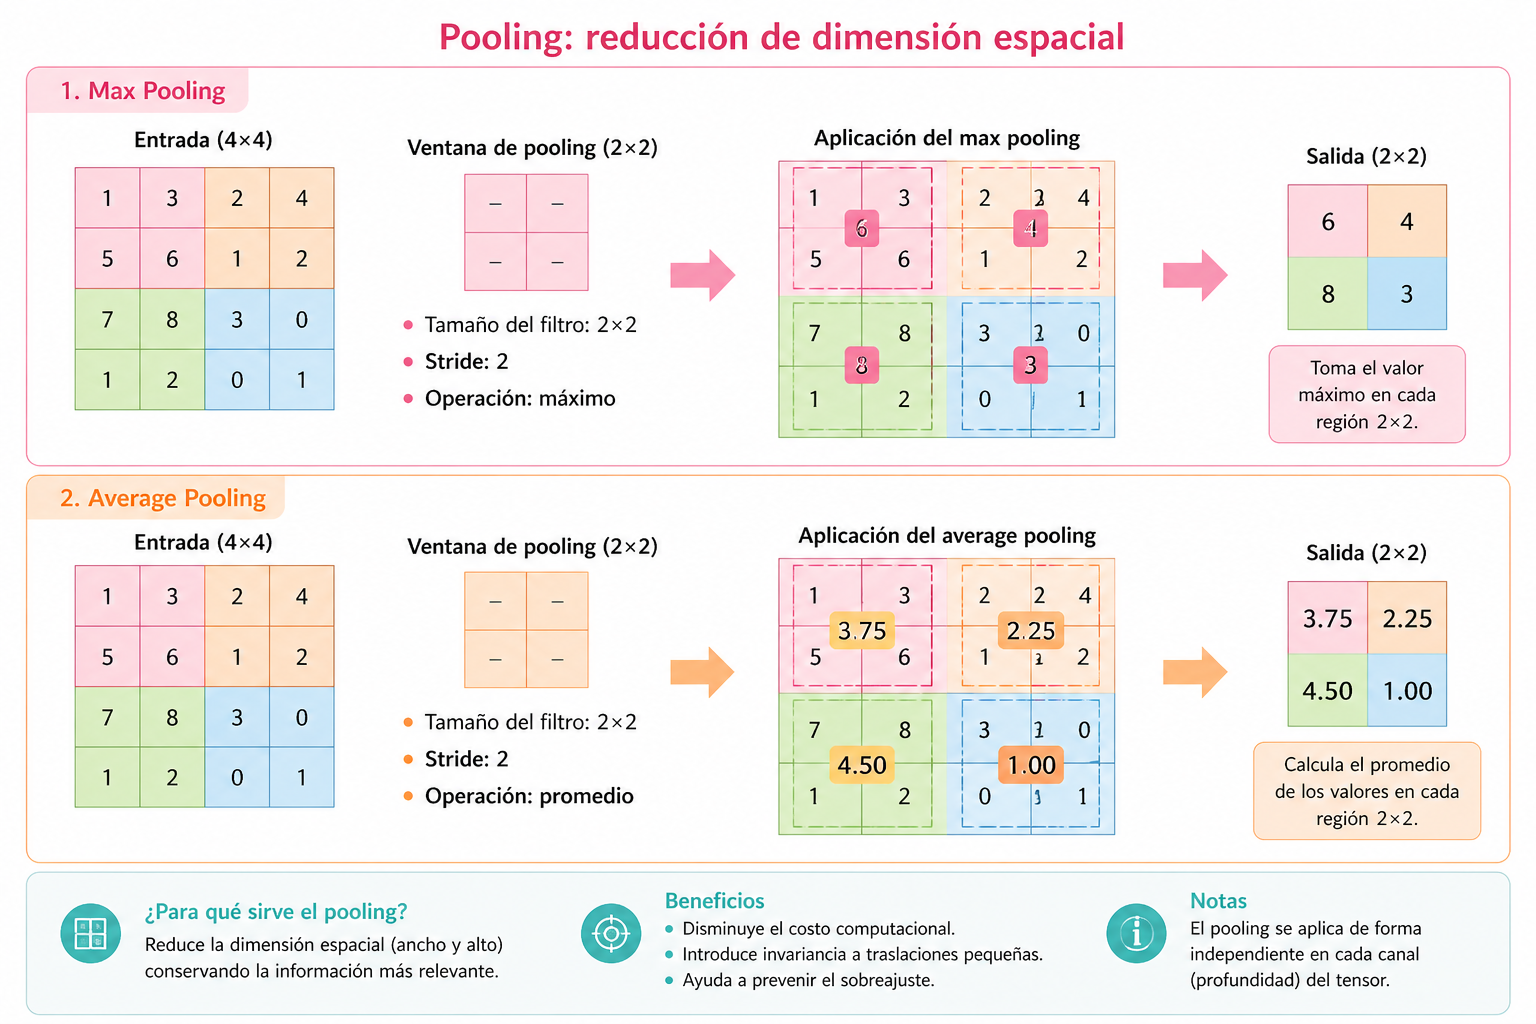
\includegraphics[width=0.8\linewidth,height=\textheight,keepaspectratio]{Imagenes_tesis/img_pooling.png}

}

\caption{\label{fig-pooling}}

\end{figure}%

\subsection{Propiedades}\label{propiedades}

El pooling presenta las siguientes propiedades:

\begin{itemize}
\tightlist
\item
  Reduce la dimensionalidad espacial, disminuyendo el costo
  computacional\\
\item
  Introduce una cierta invariancia a traslaciones pequeñas\\
\item
  Opera de forma independiente en cada canal
\end{itemize}

\subsection{Interpretación}\label{interpretaciuxf3n}

El pooling puede interpretarse como una forma de resumen local de la
información. En el caso del max pooling, se selecciona la característica
más prominente dentro de cada región, mientras que el average pooling
produce una media de las intensidades.

En arquitecturas profundas, el pooling contribuye a la construcción de
representaciones más abstractas, al reducir progresivamente la
resolución espacial.

\section{Capas completamente
conectadas}\label{capas-completamente-conectadas}

Las capas completamente conectadas (\emph{Fully Connected}, FC)
constituyen la etapa final de una red neuronal convolucional. Su función
es combinar las características extraídas por las capas anteriores para
realizar la tarea de clasificación o regresión.

\subsection{Vectorización de la
entrada}\label{vectorizaciuxf3n-de-la-entrada}

Sea:

\[
X \in \mathbb{R}^{H \times W \times C}
\]

la salida de la última capa convolucional. Esta se transforma en un
vector mediante una operación de vectorización:

\begin{equation}\phantomsection\label{eq-vectorizacion-fc}{
x = \mathrm{vec}(X) \in \mathbb{R}^{HWC}
}\end{equation}

\subsection{Transformación afín}\label{transformaciuxf3n-afuxedn}

La capa completamente conectada aplica una transformación lineal seguida
de un sesgo:

\begin{equation}\phantomsection\label{eq-fc-lineal}{
z = Wx + b
}\end{equation}

donde:

\begin{itemize}
\tightlist
\item
  \(W \in \mathbb{R}^{k \times HWC}\) es la matriz de pesos\\
\item
  \(b \in \mathbb{R}^{k}\) es el vector de sesgos\\
\item
  \(k\) es el número de neuronas en la capa
\end{itemize}

\subsection{Aplicación de la función de
activación}\label{aplicaciuxf3n-de-la-funciuxf3n-de-activaciuxf3n}

La salida de la capa está dada por:

\begin{equation}\phantomsection\label{eq-fc-activacion}{
y = \sigma(z)
}\end{equation}

donde \(\sigma\) es una función de activación aplicada componente a
componente.

\subsection{Interpretación}\label{interpretaciuxf3n-1}

Las capas completamente conectadas pueden interpretarse como
clasificadores que operan sobre las características extraídas por la red
convolucional. En particular, cada neurona combina toda la información
disponible en la representación vectorizada.

Esto contrasta con las capas convolucionales, donde la conectividad es
local.

\subsection{Clasificación}\label{clasificaciuxf3n}

En problemas de clasificación multiclase, la última capa suele utilizar
la función \emph{softmax}, definida como:

\begin{equation}\phantomsection\label{eq-softmax}{
\text{softmax}(z_i) =
\frac{e^{z_i}}{\sum_{j=1}^{k} e^{z_j}}
}\end{equation}

Esta función transforma el vector \(z\) en una distribución de
probabilidad sobre las clases.

\subsection{Propiedades}\label{propiedades-1}

Las capas completamente conectadas presentan las siguientes
características:

\begin{itemize}
\tightlist
\item
  Conectividad global: cada neurona está conectada con todas las
  entradas\\
\item
  Alta capacidad de representación\\
\item
  Mayor número de parámetros en comparación con capas convolucionales
\end{itemize}

\subsection{Observación}\label{observaciuxf3n}

Debido al elevado número de parámetros, las capas completamente
conectadas son más propensas al sobreajuste. Por esta razón, en
arquitecturas modernas, su uso se reduce o se reemplaza parcialmente
mediante técnicas como \emph{global average pooling}.

\section{Función de pérdida}\label{funciuxf3n-de-puxe9rdida}

La función de pérdida (\emph{loss function}) cuantifica la discrepancia
entre las predicciones del modelo y los valores reales. Constituye el
criterio fundamental que guía el proceso de entrenamiento, ya que
permite evaluar la calidad de las predicciones y definir un objetivo de
optimización.

\subsection{Definición general}\label{definiciuxf3n-general}

Sea \(f_\theta(x)\) la salida del modelo para una entrada \(x\), y sea
\(y\) la etiqueta real asociada. Una función de pérdida se define como:

\[
\mathcal{L}(f_\theta(x), y)
\]

donde \(\mathcal{L} : \mathbb{R}^k \times \mathbb{R}^k \to \mathbb{R}\)
mide el error entre la predicción y el valor objetivo.

Dado un conjunto de datos \(\{(x_i, y_i)\}_{i=1}^{N}\), la función de
costo global se define como:

\begin{equation}\phantomsection\label{eq-risk}{
J(\theta) = \frac{1}{N} \sum_{i=1}^{N} \mathcal{L}(f_\theta(x_i), y_i)
}\end{equation}

\subsection{Clasificación multiclase: Entropía
cruzada}\label{clasificaciuxf3n-multiclase-entropuxeda-cruzada}

En problemas de clasificación multiclase, la función de pérdida más
utilizada es la entropía cruzada (\emph{cross-entropy}).

Sea \(p = f_\theta(x)\) la salida del modelo después de aplicar la
función \emph{softmax}, y sea \(y\) un vector one-hot que representa la
clase verdadera. La pérdida se define como:

\begin{equation}\phantomsection\label{eq-cross-entropy}{
\mathcal{L}(p, y) = - \sum_{j=1}^{k} y_j \log(p_j)
}\end{equation}

Dado que \(y\) es un vector one-hot, esta expresión se reduce a:

\[
\mathcal{L}(p, y) = -\log(p_{y})
\]

donde \(p_y\) es la probabilidad asignada a la clase correcta.

\subsection{Interpretación
probabilística}\label{interpretaciuxf3n-probabiluxedstica}

La entropía cruzada puede interpretarse como una medida de divergencia
entre la distribución verdadera \(y\) y la distribución predicha \(p\).
Minimizar esta función equivale a maximizar la probabilidad de observar
los datos bajo el modelo.

Desde un punto de vista estadístico, este enfoque corresponde al método
de máxima verosimilitud.

\subsection{Caso de regresión: Error cuadrático
medio}\label{caso-de-regresiuxf3n-error-cuadruxe1tico-medio}

En problemas de regresión, una función de pérdida común es el error
cuadrático medio (\emph{Mean Squared Error}, MSE), definido como:

\begin{equation}\phantomsection\label{eq-mse}{
\mathcal{L}(f_\theta(x), y) = \| f_\theta(x) - y \|^2
}\end{equation}

Esta función penaliza de manera más severa los errores grandes, lo que
favorece ajustes más precisos.

\subsection{Relación con el
entrenamiento}\label{relaciuxf3n-con-el-entrenamiento}

El objetivo del entrenamiento consiste en encontrar los parámetros
\(\theta\) que minimizan la función de costo global:

\begin{equation}\phantomsection\label{eq-opt}{
\theta^* = \arg\min_{\theta} J(\theta)
}\end{equation}

Este problema se resuelve típicamente mediante métodos de optimización
iterativos, como el descenso por gradiente y sus variantes.

\section{Entrenamiento}\label{entrenamiento}

El entrenamiento de una red neuronal convolucional consiste en ajustar
los parámetros \(\theta\) del modelo con el objetivo de minimizar la
función de pérdida definida previamente.

Dado un conjunto de datos \(\{(x_i, y_i)\}_{i=1}^{N}\), el problema de
entrenamiento puede formularse como:

\begin{equation}\phantomsection\label{eq-entrenamiento}{
\min_{\theta} J(\theta) = \frac{1}{N} \sum_{i=1}^{N} \mathcal{L}(f_\theta(x_i), y_i)
}\end{equation}

\subsection{Descenso por gradiente}\label{descenso-por-gradiente}

El método más utilizado para resolver este problema es el descenso por
gradiente. Este consiste en actualizar iterativamente los parámetros en
la dirección opuesta al gradiente de la función de pérdida:

\begin{equation}\phantomsection\label{eq-gradient-descent}{
\theta \leftarrow \theta - \eta \nabla_{\theta} J(\theta)
}\end{equation}

donde:

\begin{itemize}
\tightlist
\item
  \(\eta > 0\) es la tasa de aprendizaje (\emph{learning rate}),
\item
  \(\nabla_{\theta} J(\theta)\) es el gradiente de la función de costo
  respecto a los parámetros.
\end{itemize}

\subsection{Interpretación}\label{interpretaciuxf3n-2}

El gradiente \(\nabla_{\theta} J(\theta)\) indica la dirección de mayor
crecimiento de la función de pérdida. Por lo tanto, al desplazarse en la
dirección opuesta, se busca reducir el valor de la función.

El proceso iterativo continúa hasta alcanzar un mínimo local de la
función de costo.

\subsection{Regla de la cadena y
retropropagación}\label{regla-de-la-cadena-y-retropropagaciuxf3n}

El cálculo del gradiente en redes neuronales profundas se realiza
mediante el algoritmo de retropropagación (\emph{backpropagation}), el
cual se basa en la aplicación sistemática de la regla de la cadena.

Sea una red expresada como:

\[
f_\theta = f^{(L)} \circ \cdots \circ f^{(1)}
\]

el gradiente de la pérdida respecto a los parámetros de una capa \(l\)
se obtiene propagando el error desde la salida hacia las capas
anteriores.

Este procedimiento permite calcular eficientemente:

\[
\nabla_{\theta^{(l)}} J(\theta)
\]

para cada capa \(l\) de la red.

\section{Regularización}\label{regularizaciuxf3n}

En el entrenamiento de redes neuronales, es común que el modelo se
ajuste excesivamente a los datos de entrenamiento, fenómeno conocido
como \emph{sobreajuste} (\emph{overfitting}). En este caso, el modelo
presenta un buen desempeño en los datos de entrenamiento, pero
generaliza pobremente a datos no vistos.

La regularización consiste en un conjunto de técnicas diseñadas para
mejorar la capacidad de generalización del modelo.

\subsection{Sobreajuste}\label{sobreajuste}

El sobreajuste ocurre cuando el modelo aprende no solo las
características relevantes del problema, sino también el ruido presente
en los datos. Esto suele suceder cuando el modelo tiene una alta
capacidad de representación en relación con la cantidad de datos
disponibles.

\subsection{Penalización de parámetros (Weight
Decay)}\label{penalizaciuxf3n-de-paruxe1metros-weight-decay}

Una estrategia común consiste en añadir un término de penalización a la
función de costo:

\begin{equation}\phantomsection\label{eq-regularizacion-l2}{
J(\theta) = \frac{1}{N} \sum_{i=1}^{N} \mathcal{L}(f_\theta(x_i), y_i) + \lambda \|\theta\|^2
}\end{equation}

donde:

\begin{itemize}
\tightlist
\item
  \(\lambda > 0\) es el parámetro de regularización\\
\item
  \(\|\theta\|^2\) es la norma cuadrática de los parámetros
\end{itemize}

Este término penaliza valores grandes de los parámetros, favoreciendo
modelos más simples.

\subsection{Dropout}\label{dropout}

El \emph{dropout} es una técnica que consiste en desactivar
aleatoriamente un subconjunto de neuronas durante el entrenamiento.

Formalmente, puede interpretarse como la multiplicación de la salida de
una capa por una máscara aleatoria \(m\), donde cada componente cumple:

\[
m_i \sim \text{Bernoulli}(p)
\]

De este modo, la salida efectiva es:

\[
\tilde{h} = m \odot h
\]

donde \(\odot\) denota el producto elemento a elemento.

Esta técnica reduce la dependencia entre neuronas y mejora la capacidad
de generalización.

\section{Optimización}\label{optimizaciuxf3n}

El proceso de entrenamiento de una red neuronal implica la resolución de
un problema de optimización en alta dimensión. En la práctica, este
problema se aborda mediante métodos iterativos basados en gradiente.

\subsection{Descenso por gradiente estocástico
(SGD)}\label{descenso-por-gradiente-estocuxe1stico-sgd}

En lugar de utilizar todo el conjunto de datos en cada iteración, el
\emph{Stochastic Gradient Descent} (SGD) emplea subconjuntos
(mini-batches):

\[
\theta \leftarrow \theta - \eta \nabla_{\theta} \mathcal{L}(f_\theta(x_i), y_i)
\]

Este enfoque reduce el costo computacional y permite actualizaciones más
frecuentes.

\subsection{Mini-batch gradient
descent}\label{mini-batch-gradient-descent}

Una generalización del SGD consiste en utilizar lotes de tamaño
intermedio:

\begin{equation}\phantomsection\label{eq-minibatch}{
\theta \leftarrow \theta - \eta \frac{1}{B} \sum_{i=1}^{B} \nabla_{\theta} \mathcal{L}(f_\theta(x_i), y_i)
}\end{equation}

donde \(B\) es el tamaño del lote.

\subsection{Métodos adaptativos}\label{muxe9todos-adaptativos}

Existen métodos de optimización que ajustan automáticamente la tasa de
aprendizaje para cada parámetro. Uno de los más utilizados es
\emph{Adam}.

El algoritmo Adam combina ideas de momento y escalamiento adaptativo del
gradiente. De manera simplificada, realiza actualizaciones de la forma:

\[
\theta \leftarrow \theta - \eta \frac{m_t}{\sqrt{v_t} + \epsilon}
\]

donde:

\begin{itemize}
\tightlist
\item
  \(m_t\) es el promedio exponencial de los gradientes\\
\item
  \(v_t\) es el promedio exponencial de los gradientes al cuadrado\\
\item
  \(\epsilon\) es un término de estabilidad numérica
\end{itemize}

\subsection{Tasa de aprendizaje}\label{tasa-de-aprendizaje}

La tasa de aprendizaje \(\eta\) controla la magnitud de las
actualizaciones. Su elección es crucial:

\begin{itemize}
\tightlist
\item
  valores pequeños producen convergencia lenta\\
\item
  valores grandes pueden causar inestabilidad
\end{itemize}

En la práctica, se utilizan esquemas de decaimiento de la tasa de
aprendizaje.

\bookmarksetup{startatroot}

\chapter{}\label{section}




\end{document}
